\documentclass{article}
\usepackage{amsmath,amssymb}
\usepackage{graphicx}
\usepackage[top=3cm, bottom=3cm, right=3cm, left=3cm]{geometry}

\begin{document}

\newpage{}
\tableofcontents
\newpage{}

\newpage
\section{Teoria de Colas}

\subsection{Introducción}
\subsubsection{Conceptos basicos}

Los fenónmenos de \textit{congestión} o \textit{espera} estan relacionados con los sistemas estocasticos y pueden describirse como sistemas integrados por uno o mas \textit{centros de atención} donde se brinda un servicio.
Cada centro de atención es, a su vez, un sistema constituido por:

\begin{itemize}
    \item \textit{canales (ó servidores)}: Entidades que prestan el servicio. 
    \item \textit{clientes (ó usuario)}: Entidades que reciben el servicio. 
\end{itemize}

    \begin{figure}[h!]
        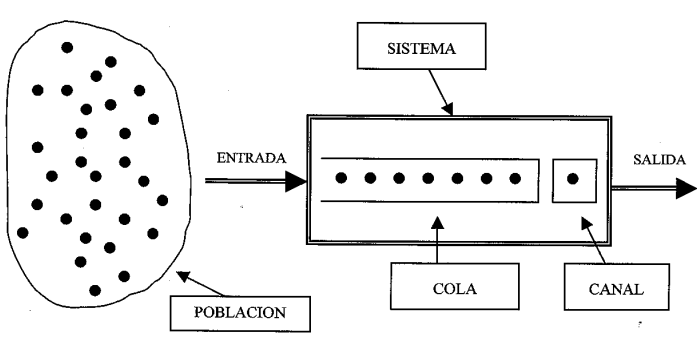
\includegraphics[width=\linewidth]{imagenes/modelo_sistema.png}
    \end{figure}

Las colas se forman cuando la demande de un servicio dado en un intervalo de tiempo exede la capacidad para proveerlo.
El administrador del sistema de establecer un balance apropiado entre los costos asociados a la espera de los usuarios y los costos vinculados con la mejora del servicio (mas servidores, mayor velocidad de atención, etc).
En la mayoria de los procesos de atención, los tiempos entre arribos de clientes y los tiempos de los servicios no son predecibles. En estas condiciones se aplica la denomida \textit{teoría de colas} para determinar el comportamiento del sistema bajo diferentes alternativas.
Se estudiaran aquellos sistemas que describan los procesos mas generales y que son los que pueden formularse como \textit{cadenas markovianas de primer orden}. Se analisaran los sistemas en regimen permanente, a través de variables tales como la \textit{longitud promedio de la cola}, el \textit{tiempo de espera promedio} del cliente para recibir el servicio, el \textit{tiempo de permanencia} en el sistema, etc. 
Esta información, junstamente con los costos relevantes, permitira al directivo determinar los valores apropiados de las variables de decisión. Las variables de decisión tipicas en los sistemas de colas estan referidas a la \textit{capacidad de servicio}(numero de canales, velocidad de canales) ó la \textit{capadidad de espera} (número de lugares).

    \begin{figure}[h!]
        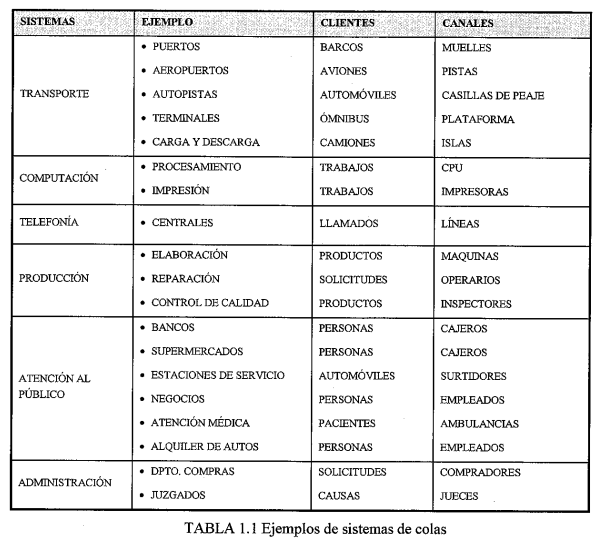
\includegraphics[width=\linewidth]{imagenes/ejemplo_sistemas_colas.png}
    \end{figure}

La \textbf{población} es el conjunto de usuario potenciales del sistema. Puede ser finito o infini  to.

En los \textbf{arribos} la llegada de los clientes puede ser deterministica o aleatoria. A menudo los intervalos entre llegadas son estadisticamente independientes y estacionarios a lo largo de prolongados periodos de tiempo, por lo que se puede suponer poissonianos.

La \textbf{impaciencia} se verifica cuando algunos usuarios que arriban al sistema se retiran sin recibir el servicio porque consideran que el tiempo de espera sera suficientemente largo. Se distingen dos tiempos de impaciencia:
\begin{enumerate}
    \item \textbf{Rechazo ($\overline{R}$)}: Un cliente que arriba, observa la cantidad de gente que esta delante de él esperando y en función de ello toma la decisión de incorporarse o no al sistema. \textbf{En la materia se trata unicamente este tipo de impaciencia}.
    \item \textbf{Abandono ($\overline{A}$)}: Un cliente que arriba, ingresa al sistema y al cabo de un tiempo toma la decisión de seguir esperando o no.
\end{enumerate}

La \textbf{capacidad} es el número máximo de clientes que puede permanecer en el sistema simultaneamente(en espera y atendiéndose).

Para el \textbf{modo de arribo} los usuarios pueden llegar en forma individual o en masa(modo batch). En la mayoria de los sistemas que estudiaremos se hará la suposición de que los procesos de llegado son del tipo Poisson, lo que implica \textit{arribos individuales}. Se puede considerar el arribo de grupos como clientes individuales. 

Para la \textbf{prioridad de atención}, existen diversos criterios de atención en lo que se refiere al orden de selección de clientes para brindar el servicio. Ellos son:

\begin{itemize}
    \item \underline{Base FIFO{(first in, first out)}}: Los clientes se atienden según el orden de llegada.
    \item \underline{Base LIFO{(last in, first out)}}: El último individuo que arriba es el primero en ser atendido.
    \item \underline{Base SIRO\textit{(service in random order)}}: Es una selección aleatoria de los clientes para brindales el servicio. 
    \item \underline{Base con PRIORIDADES}: Se establecen criterios de atención conforme a los atributos de los clientes. 
\end{itemize}

La \textbf{duración del servicio} es el tiempo requerido por un canal para atender un cliente. Puede ser una variable deterministica o aleatoria con distribución de probabilidad conocida.

En el \textbf{modo de atención} un canal puede servicio de forma individual o multiples(en masa). En la mayoria de los sistemas reales, el modo de atención es individual.

Los \textbf{procesos poisson} son markovianos y tienen dos distribuciones que lo describen:
\begin{enumerate}
    \item La distribución Poisson, en donde la variable es el número de eventos que se producen en un intervalo determinado de continuo.
    \item La distribución Gamma, en la que la variable es el intervalo de continuo necesario para que se verifique un número determinado de eventos. Partucularmente, cuando la variable es el intervalo de tiempo de continuo necesario para que se verifique \textit{un solo evento}, la distribución es conocida como \textbf{distribución Exponencial}. 
\end{enumerate}

\underline{Distribución Poisson}
La probabilidad de que se produzcan "n" eventos en un intervalo "t" estada dada por:
\begin{equation}
    p(n)= \frac{( \lambda \Delta t) ^ { n } \cdot e^{ - \lambda \Delta t}}{n!}
\end{equation}
siendo \(n=1,2,...\) y \( \lambda > 0\)
La media de esta distribución es \(a = \lambda . t\) y el desvio estandar \(\sigma=\sqrt{\lambda t}\).

\underline{Distribución Gamma}
La función distribución de probabilidad de la \textbf{distribución exponencial} esta dada por la siguiente expresión:

\begin{equation}
    f(t) = \lambda . e^{-\lambda t}
\end{equation}
cuya media es \(\frac{1}{\lambda}\)
y cuyo desvio estandar es \(\frac{1}{\lambda}\)

Si el proceso de arribos es de tipo Poisson significa que la variable "tiempo entre dos arribos sucesivos" tiene distribución \textit{exponencial} y la variable "numero de clientes que arriban por unidad de tiempo" tiene distribución \textit{Poisson}.

\textbf{Ingresos y egresos de clientes}: 
En los sistemas de capacidad finita o de población impaciente, no todos los clientes que arriban al sistema ingresan.
\begin{itemize}
    \item $\overline{\lambda}$: Número promedio de clientes que ingresan efectivamente al sistema.
    \item $\overline{R}$: Número promedio de rechazados(es decir, que no ingresan al sistema).
    \item $\overline{\mu}$: Número promedio de clientes atendidos que egresan del sistema.
    \item $\overline{A}$: Tasa de clientes que ingresaron al sistema pero que decidieron abandonarlo sin recibir el servicio.
\end{itemize}

\newpage
\textbf{Estructuras de sistemas simples}:
\begin{figure}[h!]
    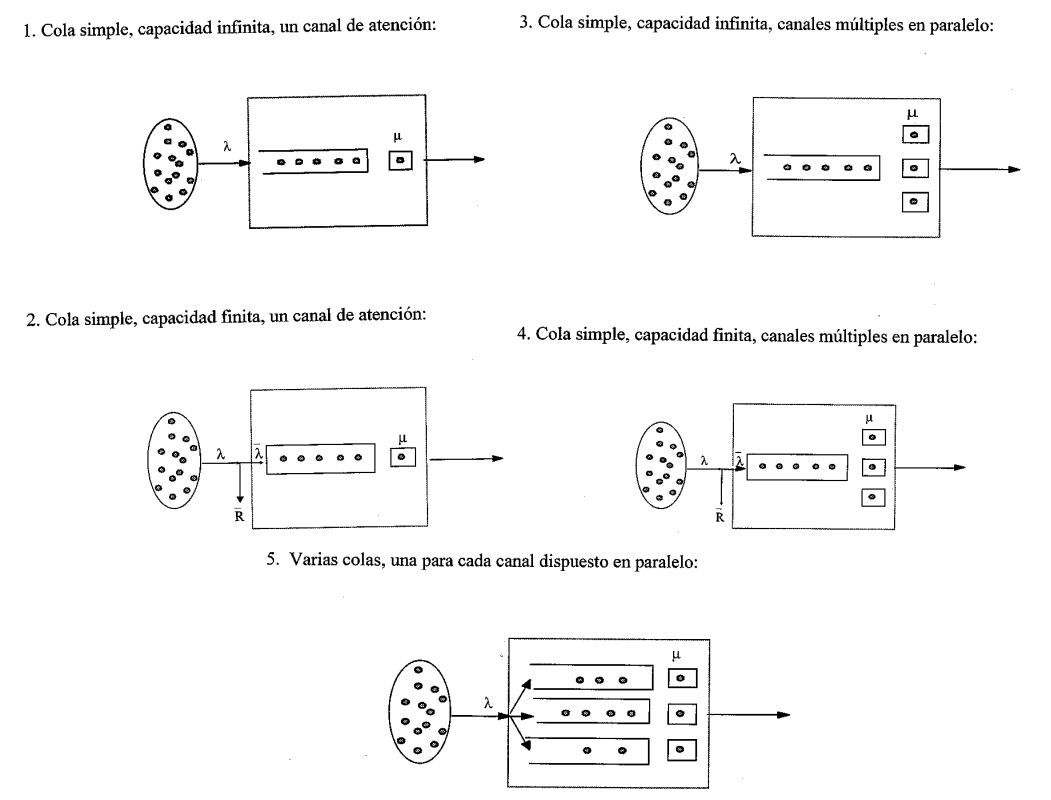
\includegraphics[width=\linewidth]{imagenes/estructuras_simples.png}
\end{figure}

\newpage
\subsubsection{Notación Kendall}
Especifica las caracteristicas descriptivas de una unidad operativa de un sistema de colas. Es una notación de 6 posiciones:
\begin{equation}
    1 / 2 / 3 / 4 / 5 / 6    
\end{equation}

\begin{enumerate}
    \item La posición 1 se refiere al patrón de arribos al sistema. Puede ser:
    \begin{itemize}
        \item P: Proceso de Poisson.
        \item D: Proceso deterministico.
        \item G: Cualquier otro proceso.
    \end{itemize}
    \item La posición 2 indica el patrón de servicio en los canales.
    \begin{itemize}
        \item P: Proceso de Poisson.
        \item D: Proceso deterministico.
        \item G: Cualquier otro proceso.
    \end{itemize}
    \item La posición 3 indica el número de canales de atención dispuestos en paralelo en la unidad operativa.
    \item La posición 4 indica la capacidad de la unidad operativa del sistema(Los que pueden esperar en la cola mas los que se pueden atender). Se asume infinita y no se indica.
    \item La posición 5 indica la prioridad de atension de la cola.  Si no se especifica se asume de tipo FIFO.
    \begin{itemize}
        \item FIFO
        \item LIFO
        \item SIRO
        \item G: Cualquier otra modalidad de atención
    \end{itemize}
    \item La última posición (entre paréntesis) se refiere al tamaño de la población. Si no se indica, el tamaño es infinito.
\end{enumerate}

\subsubsection{Ecuacion de estado en regimen permante}

\begin{equation}
    p(n)= p(n-1) \cdot \frac{ \lambda_{n-1}}{\mu_n}
\end{equation}



\newpage
\subsubsection{Preguntas y respuestas}
\begin{itemize}
    \item ¿Qué características posee la población?
        \newline\textit{Rta: Puede ser Finita o infinita}
    \item ¿En qué consiste el fenómeno de impaciencia? ¿cuántos tipos de impaciencia hay? ¿en qué consisten?
        \newline\textit{Rta: Ver punto de impaciencia mas arriba.}
    \item ¿Qué características posee el sistema?
        \newline\textit{Rta: Dependiendo de las hipotesis, puede uno o varios canales, con una o varias colas, y la cola puede ser finita o infinita}
    \item ¿Qué se entiende por capacidad del sistema?
        \newline\textit{Rta: Es el numero máximo de clientes que pueden estar en todo el sistema}
    \item ¿Con qué notación identificamos cada uno de los ítems enunciados?
        \begin{itemize}
            \item \(L_c\): La cantidad promedio de clientes que están esperando para recibir el servicio en un determinado momento.
            \item \(L\): La cantidad promedio de clientes que se encuentran en el sistema en un determinado momento, ya sea esperando ser atendidos como atendiéndose.
            \item \(W_c\): El tiempo promedio que un cliente debe esperar para ser atendido.
            \item \(W\): El tiempo promedio que un cliente permanece en el sistema, ya sea esperando ser atendido como atendiéndose.
            \item \(\lambda\): La cantidad promedio de clientes que arriban al sistema en un determinado momento.
            \item $\overline{\lambda}$: la cantidad promedio de clientes que ingresan al sistema en un determinado momento.
            \item $\overline{\mu}$: La cantidad promedio de clientes que egresan del sistema luego de ser atendidos.
            \item \(\mu\): La velocidad promedio de atención de un canal.
            \item \(T_a\): El tiempo promedio entre arribos.
            \item \(H\): La cantidad promedio de canales ocupados.
            \item \(PA\): El porcentaje de actividad de cada canal.
        \end{itemize}
    \item ¿Cuál es la diferencia entre “la cantidad promedio de clientes que arriban al sistema en un determinado momento” y “la cantidad promedio de clientes que ingresan al sistema en un determinado momento”?
        \newline\textit{Rta: No todos los clientes que arriban al sistema, ingresan. Y por esos se diferencia los que arriban, y dentro de estos lo que finalmente ingresan.}
    \item ¿Qué significa que se encuentren en régimen permanente o estacionario?
        \newline\textit{Cuando los valores de las variables no dependen de las condiciones iniciales del sistema.}       
    \item ¿qué se indica cada una de las posiciones de la notación Kendall?
        \newline\textit{Rta: Se describen mas arriba}
    \item ¿Qué características posee el modelo \(P/P/1\)?
        \newline\textit{Se refiere a una unidad operativa de un sistema de colas con arribo Poisson, servicio Poisson, un canal, con capacidad infinita, en modalidad FIFO ya que no especifica y con población infinita}
    \item ¿Cuánto debe valer \(\rho\) en un \(P/P/1\)? ¿Por qué?
        
    \item Según el modelo \(P/P/1/N\) ¿Cuáles son sus características según la notación de Kendall?
    \item En el modelo \(P/P/1/N\), ¿debe verificarse lo mismo que en el \(P/P/1\) respecto del valor de \(\rho\)? ¿Por qué?
    \item ¿Qué ejemplos de la vida cotidiana se podrían plantear en cada uno de los modelos mencionados?
\end{itemize}

\subsection{Sistemas de un solo canal, capacidad infinita y poblacion infinita}

\underline{HIPOTESIS}
\begin{itemize}
    \item El proceso de arribos de clientes es de tipo Poisson.
    \item El proceso de servicio tambien es de tipo Poisson.
    \item El sistema se encuentra en condiciones estables.
    \item Los clientes que llegan al sistema forman una cola simple.
    \item La diciplina de atención es FIFO.
    \item Se dispone de un solo canal de atención.
    \item La capacidad del sistema es ilimitada.
    \item Los clientes que llegan al sistema no presentan impaciencia.
    \item La población de clientes potenciales del sistema es infinita.
\end{itemize}

\begin{quote}
    
\end{quote}
\end{document}

